\documentclass[border=10pt]{standalone}
% \usepackage{subfigure}
\usepackage{subcaption}
\usepackage{colortbl}
\usepackage{tikz}
\usetikzlibrary{decorations.pathmorphing, shapes, matrix, positioning}
\begin{document} 
  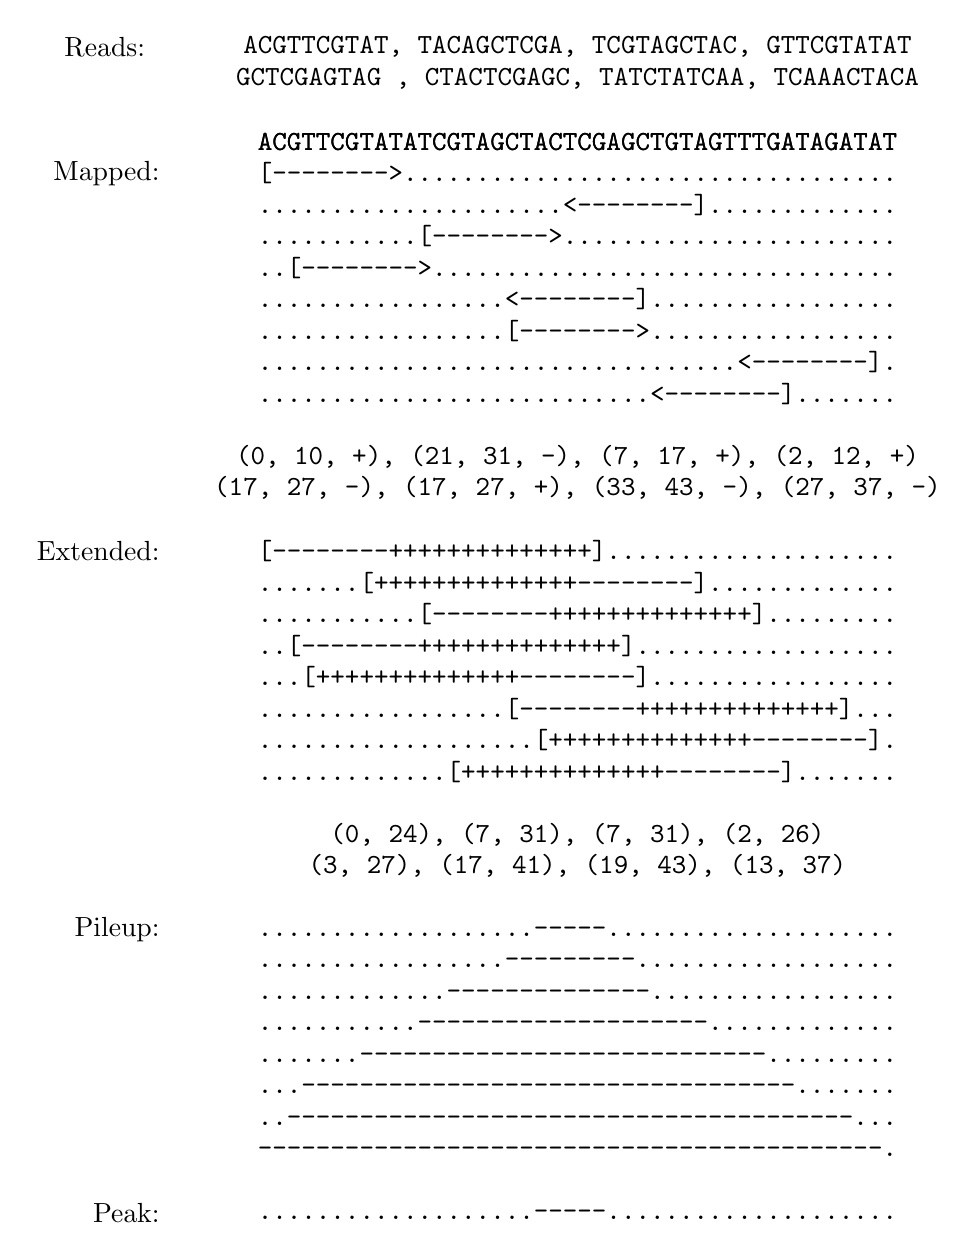
\begin{tikzpicture}[decoration={coil},
dna/.style={decorate, thick, decoration={aspect=0, segment length=1.0cm}},
protein/.style={ellipse, draw=white, minimum width=1cm, minimum height=1cm}]
\tikzstyle{seq}=[font=\ttfamily]
      \def\fy{0.4}
      \node[seq] (reads) at (3, 3*\fy) {ACGTTCGTAT, TACAGCTCGA, TCGTAGCTAC, GTTCGTATAT};
      \node[seq] at (3, 2*\fy) {GCTCGAGTAG , CTACTCGAGC, TATCTATCAA, TCAAACTACA};
 \def\fy{0.4}
%DNA
\node[seq] at (3,0)      {ACGTTCGTATATCGTAGCTACTCGAGCTGTAGTTTGATAGATAT};
\node[seq] (mapped) at (3,-1*\fy) {[-------->..................................};
\node[seq] at (3,-2*\fy) {.....................<--------].............};
\node[seq] at (3,-3*\fy) {...........[-------->.......................};
\node[seq] at (3,-4*\fy) {..[-------->................................};
\node[seq] at (3,-5*\fy) {.................<--------].................};
\node[seq] at (3,-6*\fy) {.................[-------->.................};
\node[seq] at (3,-7*\fy) {.................................<--------].};
\node[seq] at (3,-8*\fy) {...........................<--------].......};
% 0, 7, 11, 2,
% 3, 17, 19, 13
\node[seq] at (3, -10*\fy) {(0, 10, +), (21, 31, -), (7, 17, +), (2, 12, +)};
\node[seq] at (3, -11*\fy) {(17, 27, -), (17, 27, +), (33, 43, -), (27, 37, -)};

\node[seq] at (3, 0)      {ACGTTCGTATATCGTAGCTACTCGAGCTGTAGTTTGATAGATAT};
\node[seq] (extended) at (3,-13*\fy) {[--------++++++++++++++]....................};
\node[seq] at (3,-14*\fy) {.......[++++++++++++++--------].............};
\node[seq] at (3,-15*\fy) {...........[--------++++++++++++++].........};
\node[seq] at (3,-16*\fy) {..[--------++++++++++++++]..................};
\node[seq] at (3,-17*\fy) {...[++++++++++++++--------].................};
\node[seq] at (3,-18*\fy) {.................[--------++++++++++++++]...};
\node[seq] at (3,-19*\fy) {...................[++++++++++++++--------].};
\node[seq] at (3,-20*\fy) {.............[++++++++++++++--------].......};

\node[seq] at (3, -22*\fy) {(0, 24), (7, 31), (7, 31), (2, 26)};
\node[seq] at (3, -23*\fy) {(3, 27), (17, 41), (19, 43), (13, 37)};


\node[seq] (pileup) at (3,-25*\fy) {...................-----....................};
\node[seq] at (3,-26*\fy) {.................---------..................};
\node[seq] at (3,-27*\fy) {.............--------------.................};
\node[seq] at (3,-28*\fy) {...........--------------------.............};
\node[seq] at (3,-29*\fy) {.......----------------------------.........};
\node[seq] at (3,-30*\fy) {...----------------------------------.......};
\node[seq] at (3,-31*\fy) {..---------------------------------------...};
\node[seq] at (3,-32*\fy) {-------------------------------------------.};

\node[seq] (peak) at (3,-34*\fy) {...................-----....................};

\node[left=of reads] {Reads:};
\node[left=of mapped] {Mapped:};
\node[left=of extended] {Extended:};
\node[left=of pileup] {Pileup:};
\node[left=of peak] {Peak:};
% \node[seq] at (3, -25*\fy) {+.++..+...+.+...+.+...-.--..-...-.-...-.-..};

\end{tikzpicture}
% \begin{tabular}{| r | r | r | r |}
%   \hline
%   Interval & Extended & Sorted\\
%   \hline
%   (0, 10, +)  & (0, 24)  & (0, 24) \\
%   (21, 31, -) & (7, 31)  & (2, 26) \\
%   (7, 17, +)  & (7, 31)  & (3, 27) \\
%   (2, 12, +)  & (2, 26)  & (7, 31) \\
%   (17, 27, -) & (3, 27)  & (7, 31) \\
%   (17, 27, +) & (17, 41) & (13, 37)\\
%   (33, 43, -) & (19, 43) & (17, 41)\\
%   (27, 37, -) & (13, 37) & (19, 43)\\
%   \hline
%               & $O(n)$   & $O(n \log n)$\\
%   \hline
% \end{tabular}
% \begin{tabular}{|r|r|r|r|r|}
%   \hline
%   Index & Diff & Value & P-value & Peak \\
%   \hline
%   0  & 1  & 1 & 0.93 & 0 \\
%   2  & 1  & 2 & 0.81 & 0 \\
%   3  & 1  & 3 & 0.63 & 0 \\
%   7  & 2  & 5 & 0.27 & 0 \\
%   13 & 1  & 6 & 0.15 & 0 \\
%   17 & 1  & 7 & 0.08 & 0 \\
%   19 & 1  & 8 & 0.03 & 1 \\
%   24 & -1 & 7 & 0.08 & 0 \\
%   26 & -1 & 6 & 0.15 & 0 \\
%   27 & -1 & 5 & 0.27 & 0 \\
%   31 & -2 & 3 & 0.63 & 0 \\
%   37 & -1 & 2 & 0.81 & 0 \\
%   41 & -1 & 1 & 0.93 & 0 \\
%   43 & -1 & 0 & 0.99 & 0 \\
%   \hline
% \end{tabular}
% yielding the interval $\left[19, 24\right)$ as the only peak.
% 
% In a real experiment, more intervals would be yielded which would be affected by noise in the experiment. 
% In order to reduce the effect of noise, two postprocessing steps are performed. First, small gaps between intervals are removed, then small peaks are removed:
% 
% \begin{tabular}{| r | r | r | r |}
%   \hline
%   Interval & Small Gaps Filled & Small Peaks Removed \\
%   \hline
%   (121, 125) & \textcolor{red}{(121, 125)} &  \\
%   (142, \textcolor{red}{147)} & (142,      & (142, \\
%   \textcolor{red}{(151, } 166) & 166)    & 166)\\
%   (172, 200) & (172, 200) & (172, 200) \\
%   \hline
% \end{tabular}
% \clearpage
% 
\end{document}

%%% Local Variables:
%%% mode: latex
%%% TeX-master: t
%%% End:
